\section{Three Task Result}

We will now extend the above idea to three tasks. In this scenario, let our tasks be denoted as $A$, $B$, and $C$. Task A produces output that is consumed by task $B$, which in turn produces output that is consumed by task $C$. Here we will now focus on a maximum staleness for the input which was used by $B$ to in turn produce the output that $C$ uses. In other words, we want to limit the staleness of the output of $A$ that is eventually used by $C$.

In this scenario we have a new requirement, defined similarly to the two task scenario. For this scenario, define $d_{A \to C}$ as the maximum age of the data produced by task $A$ that is used by task $C$. Note that we are not making any assumptions about when a job of task $B$ is executed between the jobs of tasks $A$ and task $C$. The formalization is similar to the two task scenario:

\begin{equation*}
	\begin{aligned}
		& \text{Given}
		& & E^*_A, E^*_B, E^*_C, P_C \text{ and } d_{A \to C} \\
		& \text{Find}
		& & P_A \text{ and } P_B \\
		& \text{That Minimizes}
		& & U(T) \\
		& \text{Subject To}
		& & \forall i, r^i_C - f_B^{C_B(r^i_C)} + E^u_B + r_B^{C_B(r^i_C)} - f_A^{C_A(r_B^{C_B(r^i_C)})} \leq d_{A \to C} \\
		%& & \text{ and } & \forall i, r^i_C - f_A^{C_A(r^i_B)} \leq d_{A \to C}\\
	\end{aligned}
\end{equation*}

The execution of the three tasks is outlined in the figure \ref{fig:3Tasks}.

\begin{figure}[!ht]
	\centering
	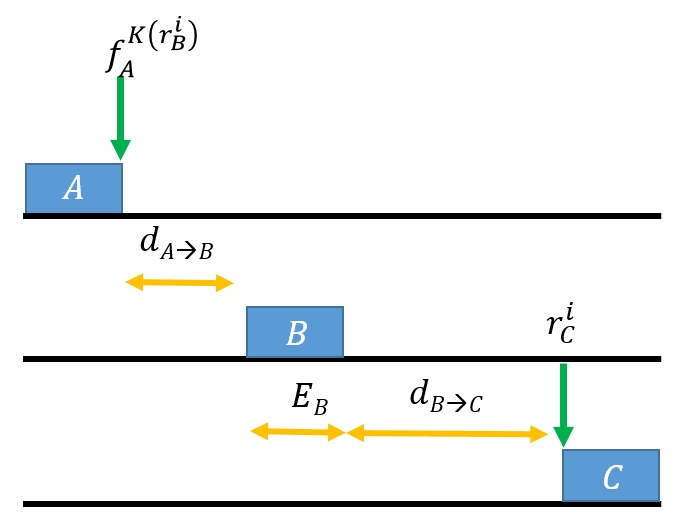
\includegraphics[width=2.5in]{figures/3TaskMaxStaleness}
	\caption{Maximum Staleness Scenario for Data from Task A.}
	\label{fig:3Tasks}
\end{figure}

Figure \ref{fig:3Tasks} labels the several intervals in the execution of the three tasks. Note how between tasks $A$ and $B$ and between tasks $B$ and $C$ we've added local freshness constraints. By meeting these two freshness constraints before and after the execution of task $B$, the freshness of data from task $A$ to task $C$ is ensured. Note that these added constraints will not be present in our final solution. They are added here to allow us to introduce Lemma 1 while being able to consider task B (considering just $d_{A \to C}$ would not guarantee that task $B$ is ran between $A$ and $C$). These local constraints are used as free variables and are never assigned concrete values. We will optimize with regards to them and use our Lemma to determine period assignments that rely only on the end-to-end constraint and the task execution times.

Note that we have one execution of task $B$ between tasks $A$ and $C$. It is up to the scheduler to ensure this. Also note that we use $E^u_B$ in this formulation. This works fine if task $B$ runs without preemption. Since we do not know the scheduling in our system, this is not guaranteed. If task $B$ may run with preemption, $E_B$ should be inflated to task $B$'s worst case response time (WCRT) instead. It would be job of the system designer to determine this WCRT with respect to the scheduler and other tasks including the ones here, which may require iteratively solving for the period/WCRT combination. We will not consider this here. In particular, probably the worst assumption with this formulation as written is that task $B$ needs to run immediately upon entering the system and without preemption.

From Figure \ref{fig:3Tasks} we can see that the maximum age of the data from task $A$ used by task $C$, $d_{A \to C}$, is the sum of three values. Concretely,
\begin{center}
	$d_{A \to C} = d_{A \to B} + E^u_B + d_{B \to C}$\\
\end{center}

We will now use our lemma to extend the two task result to this scenario. Using Lemma \ref{lem:2TaskResult} \ldots

\begin{align*}
	P_A &\leq \frac{d_{A \to B} + E^l_A}{2}\\
	& \text{ and }\\
	P_B &\leq \frac{d_{B \to C} + E^u_B}{2}\\
\end{align*}

Notice how, once again, we use the best-case execution time for the first task in the chain in order to maximize the possible staleness. Note how this will be a minor issue, as we are trying to minimize utilization but are now using the best-case execution time where a worst-case execution may occur. Since a worst-case execution will produce fresher output than a best-case under our assumption that results are produced at the end of a task, we will solve this by introducing some pessimism. For our freshness guarantee, we will use the best-case execution time whereas when calculating utilization we will use the worst-case execution time. That is, our solution will ensure freshness even in with best-case execution of the first task, while minimizing the maximum utilization the system could experience. This means that our solution for $d_{A \to B}$ will be under the assumption that the worst case-execution occurs. Hence, when we find out $d_{A \to B}$ we will subtract the difference between $E^l_A$ and$E^u_A$ so that this freshness holds even during best-case execution of task $A$, i.e., we will further decrease the period of A to account for this.

Note that in our above formulation for three task scenario, the only free variables that effect utilization are $P_A$ and $P_B$. Therefore, we can achieve the same solution by minimizing over $\left(\frac{E_A}{P_A} + \frac{E_B}{P_B}\right)$ since the utilization from task $C$ is constant. This is what we will use as our minimization objective.

Substituting the values derived from Lemma \ref{lem:2TaskResult}, we can transform the minimization objective:

\begin{align*}
	U(T) &= \left(\frac{E^u_A}{P_A} + \frac{E^u_B}{P_B}\right) &\mbox{Revised Objective}&\\
	&\geq \left(\frac{E^u_A}{\frac{d_{A \to B} + E^l_A}{2}} + \frac{E^u_B}{\frac{d_{B \to C} + E^l_B}{2}}\right) &\mbox{Substitution}&\\
	&= \left(\frac{E^u_A}{\frac{d_{A \to B} + E^l_A}{2}} + \frac{E^u_B}{\frac{d_{B \to C} + E^l_B}{2}}\right) &\mbox{Min $U(T) \to$ Max Periods}&\\
	&= \frac{2E^u_A}{d_{A \to B}+E^l_A} + \frac{2E^u_B}{d_{B \to C}+E^l_B} &\mbox{Simplification}&\\
\end{align*}

Using this modified objective, we can minimize to arrive at the following solution.

\begin{theorem}
	\label{thm:3TaskResult}
	Given $E^*_A$, $E^*_B$, $E^*_C$, and $P_C$, to minimize utilization while enforcing the freshness bound $d_{A \to C}$, choose
	\begin{align*}
		P_A &= \frac{\sqrt{\frac{E_A}{E_B}}(d_{A \to C}+E_A)}{2(1+\sqrt{\frac{E_A}{E_B}})} - \frac{(E^u_A - E^l_A)}{2}\\
		& \text{ and }\\
		P_B &= \frac{d_{A \to C}+E^u_A}{2(1+\sqrt{\frac{E^u_A}{E^u_B}})}\\
	\end{align*}
\end{theorem}

\begin{proof}
	This is a simple optimization problem that can be solved using elementary calculus methods. In particular, we will use Lagrangian multipliers. We will optimize our two controllable parameters, the local constraints, and then use these two decide upon periods for the tasks as per our Lemma.
	
	To optimize the above with our constraint of the form $x+b+y=z$, we use the following:
	\begin{center}
		$\frac{2E^u_A}{d_{A \to B}+E^u_A} + \frac{2E^u_B}{d_{B \to C}+E^u_B} + \lambda (d_{A \to C}-d_{A \to B}-E^u_B-d_{B \to C})$
	\end{center}
	
	We now take the partials with respect to our free variables, $d_{A \to B}$ and $d_{B \to C}$:
	
	\begin{align*}
		\frac{\partial}{\partial d_{A \to B}} &= -\frac{2 E^u_A}{(E^u_A+d_{A \to B})^2}-\lambda\\
		\frac{\partial}{\partial d_{B \to C}} &= -\frac{2 E^u_B}{(E^u_B+d_{B \to C})^2}-\lambda\\
	\end{align*}
	
	We set these equal to zero and solve for our $\lambda$'s \ldots
	\begin{align*}
		-\frac{2 E^u_A}{(E^u_A+d_{A \to B})^2}-\lambda &= 0 \to \lambda = -\frac{2 E^u_A}{(E^u_A+d_{A \to B})^2}\\
		-\frac{2 E^u_B}{(E^u_B+d_{B \to C})^2}-\lambda &= 0 \to \lambda = -\frac{2 E^u_B}{(E^u_B+d_{B \to C})^2}\\
	\end{align*}
	
	With two values of $\lambda$, we can form an equality, which we can use with our constraint equation to solve for $d_{A \to B}$ and $d_{B \to C}$ via a system of equations:
	
	\begin{align*}
		-\frac{2 E^u_A}{(E^u_A+d_{A \to B})^2} &= -\frac{2 E^u_B}{(E^u_B+d_{B \to C})^2}\\
		d_{A \to B}+E^u_B+d_{B \to C} &= d_{A \to C}\\
	\end{align*}
	
	We'll solve for $d_{A \to B}$ first.
	
	\begin{align*}
		-\frac{2 E^u_A}{(E^u_A+d_{A \to B})^2} &= -\frac{2 E^u_B}{(E^u_B+d_{B \to C})^2} &\mbox{}&\\
		(2 E^u_B)(E^u_A+d_{A \to B})^2 &= (2 E^u_A)(E_B+d_{B \to C})^2 &\mbox{Multiply By -1 Then Cross Multiply}&\\
		(E^u_A+d_{A \to B})^2 &= \frac{E^u_A}{E^u_B}(E^u_B+d_{B \to C})^2 &\mbox{Rearrange and Simplify}&\\
		d_{A \to B} &= \pm\sqrt{\frac{E^u_A}{E^u_B}}(E^u_B+d_{B \to C})-E^u_A &\mbox{}&\\
		&= \pm\sqrt{\frac{E^u_A}{E^u_B}}(E^u_B+d_{A \to C}-E^u_B-d_{A \to B})-E^u_A &\mbox{Substitute From Constraint}&\\
		&= \pm\sqrt{\frac{E^u_A}{E^u_B}}(d_{A \to C}-d_{A \to B})-E^u_A &\mbox{Simplify}&\\
		&= \pm\sqrt{\frac{E^u_A}{E^u_B}}d_{A \to C}-\pm\sqrt{\frac{E^u_A}{E^u_B}}d_{A \to B}-E^u_A &\mbox{}&\\
		(1+\pm\sqrt{\frac{E^u_A}{E^u_B}})d_{A \to B}&= \pm\sqrt{\frac{E^u_A}{E^u_B}}d_{A \to C}-E^u_A &\mbox{}&\\
		d_{A \to B}&= \frac{\pm\sqrt{\frac{E^u_A}{E^u_B}}d_{A \to C}-E^u_A}{(1+\pm\sqrt{\frac{E^u_A}{E^u_B}})} &\mbox{}&\\
	\end{align*}
	
	Assigning the $\pm$ both ways, we obtain two possible solutions:
	
	\begin{align*}
		d_{A \to B}&= \frac{\sqrt{\frac{E^u_A}{E^u_B}}d_{A \to C}-E^u_A}{(1+\sqrt{\frac{E^u_A}{E^u_B}})} & \text{or} & & d_{A \to B}&= \frac{-\sqrt{\frac{E^u_A}{E^u_B}}d_{A \to C}-E^u_A}{(1-\sqrt{\frac{E^u_A}{E^u_B}})} &\\
	\end{align*}
	
	And now we solve for $d_{B \to C}$ using this and the constraint equation:
	
	\begin{align*}
		d_{B \to C}&= d_{A \to C} - E^u_B - \frac{\sqrt{\frac{E^u_A}{E^u_B}}d_{A \to C}-E^u_A}{(1+\sqrt{\frac{E^u_A}{E^u_B}})} & \text{or} & & d_{B \to C}&= d_{A \to C} - E^u_B + \frac{\sqrt{\frac{E^u_A}{E^u_B}}d_{A \to C}+E^u_A}{(1-\sqrt{\frac{E^u_A}{E^u_B}})} &\\
	\end{align*}
	
	Note that we can drive up utilization arbitrarily higher (and even over-commit the system) by shortening the local constraints, and hence periods, so there is no maximum in our search space. There are also no saddle points: it is clear that from any initial value that increasing either parameter will strictly lower utilization. It follows that both of these points are minima. Now note that the second potential solutions "cheats" by using negative values. Upon inspection its easy to see how $d_{A \to B}$ can become negative when $E_A > E_B$, and is undefined when these two are equal. Upon further inspection, we see that when this is not the case, $d_{B \to C}$ will be negative instead. This minimum achieves such by using positive and negative values to cancel one another out. Since our local constraints must be positive, this is not a feasible solution and we discard it.
	
	Therefore, our solution is the first point, and we can now use our Lemma to convert these into period assignments:
	
	\begin{align*}
		P_A &= \frac{\sqrt{\frac{E^u_A}{E^u_B}}d_{A \to C}-E^u_A}{2(1+\sqrt{\frac{E^u_A}{E^u_B}})} + \frac{E^u_A}{2} &=& \frac{\sqrt{\frac{E^u_A}{E^u_B}}(d_{A \to C}+E^u_A)}{2(1+\sqrt{\frac{E^u_A}{E^u_B}})}\\
		P_B &= \frac{d_{A \to C}}{2} - \frac{\sqrt{\frac{E^u_A}{E^u_B}}d_{A \to C}-E^u_A}{2(1+\sqrt{\frac{E^u_A}{E^u_B}})} &=& \frac{d_{A \to C}+E^u_A}{2(1+\sqrt{\frac{E^u_A}{E^u_B}})}\\
	\end{align*}
	
	Finally, recall that we need the bound to hold even during best-case execution of task $A$, whereas this assumes worst-case execution. To make sure that the freshness constraint holds even under best case execution, we will base the freshness guarantee from the best-case execution time instead of the worst-case. To do this, we will reduce the period so that even under the best execution of task $A$ our freshness is ensured. Currently, we could be $E^u_A - E^l_A$ too old since we base from the worst case execution but the best base could occur. We want to shorten this freshness constraint. Recall from the two task scenario that the freshness constraint span two task periods. Therefore, if we can shorten each period by half of the above mentioned deficit to tighten our freshness guarantee. With this change, even best case execution will result in the desired freshness, and worst case executions of task $A$ will produce data more fresh than the bound.
	
	\begin{align*}
		P_A &= \frac{\sqrt{\frac{E^u_A}{E^u_B}}(d_{A \to C}+E^u_A)}{2(1+\sqrt{\frac{E^u_A}{E^u_B}})} - \frac{(E^u_A - E^l_A)}{2}\\
		P_B &= \frac{d_{A \to C}+E^u_A}{2(1+\sqrt{\frac{E^u_A}{E^u_B}})}\\
	\end{align*}
	
	This concludes our proof.
\end{proof}

Note that the solution is in regards to constants in our system that are given to us, and do not rely on our temporary local constraints in the solution, although these constraints can be extracted from the given solution.

Also note that our optimization is for worst-case utilization, and these freshness bounds may not be optimal when tasks, specifically task $A$, exhibits best-case execution. However, our goal is safety so the optimization is done for the worst-case execution.

Once again, this solution may not be schedulable. If it is not, there may or may not be a schedulable task set that produces data with the desired freshness, depending on the scheduling algorithm used. Finding the parameters in such a case may be non-trivial.

Lastly, note that this is a convex optimization problem and that we can always find an arbitrarily small periods that meets our freshness bound, i.e. we always have an interior point that satisfies our constraint and thus strictly feasible. It follows that this problem has strong duality and our solution is indeed our desired parameters.